\documentclass[UTF8,11pt,a4paper,fontset=none]{ctexart}
\usepackage[a4paper,top=1.65cm,bottom=1.65cm,left=1.85cm,right=1.85cm,headheight=15pt]{geometry}
\usepackage{fontspec,unicode-math}
\usepackage{amsmath}
\usepackage{booktabs,tabularx,array}
\usepackage[table]{xcolor}
\usepackage{graphicx,float}
\usepackage{siunitx}
\usepackage{enumitem}
\usepackage{fancyhdr}
\usepackage{caption}
\usepackage{hyperref}
\usepackage[most]{tcolorbox}
\usepackage{pdflscape}

\setmainfont{Times New Roman}
\setsansfont{Arial}
\setmonofont{Consolas}
\setmathfont{Cambria Math}
\setCJKmainfont[BoldFont=SimHei,ItalicFont=KaiTi]{SimSun}
\setCJKsansfont[BoldFont={Microsoft YaHei Bold}]{Microsoft YaHei}

\definecolor{DeepBlue}{HTML}{17324D}
\definecolor{PandaTeal}{HTML}{0B7A75}
\definecolor{WarmGold}{HTML}{C58A19}
\definecolor{Coral}{HTML}{C95F4A}
\definecolor{SoftBlue}{HTML}{EEF5F8}
\definecolor{SoftTeal}{HTML}{ECF7F5}
\definecolor{SoftGold}{HTML}{FFF7E7}
\definecolor{MidGray}{HTML}{667085}
\definecolor{LineGray}{HTML}{D5DEE5}

\hypersetup{
  colorlinks=true,
  linkcolor=DeepBlue,
  urlcolor=PandaTeal,
  pdfauthor={范子恒},
  pdftitle={PandaX-4T candidate v11 核心汇报}
}
\ctexset{
  section={format=\Large\bfseries\color{DeepBlue},number=\arabic{section},
    beforeskip=0.35em,afterskip=0.55em},
  subsection={format=\large\bfseries\color{PandaTeal},
    beforeskip=0.35em,afterskip=0.35em}
}
\pagestyle{fancy}
\fancyhf{}
\fancyhead[L]{\small\color{DeepBlue}PandaX-4T 能量重建}
\fancyhead[R]{\small\color{MidGray}candidate\_v11 核心汇报}
\fancyfoot[C]{\small\color{MidGray}\thepage}
\renewcommand{\headrulewidth}{0.4pt}

\captionsetup{font=small,labelfont=bf,labelsep=quad}
\graphicspath{{figures/}}
\setlength{\parindent}{2em}
\setlength{\parskip}{0.18em}
\setlist[itemize]{leftmargin=1.8em,itemsep=0.25em,topsep=0.25em}
\renewcommand{\arraystretch}{1.16}
\newcolumntype{Y}{>{\raggedright\arraybackslash}X}
\newcolumntype{C}[1]{>{\centering\arraybackslash}p{#1}}
\newcommand{\var}[1]{\texttt{\detokenize{#1}}}

\newtcolorbox{keybox}[1][]{enhanced,colback=SoftBlue,colframe=DeepBlue,
  boxrule=0.75pt,arc=1.6mm,left=2mm,right=2mm,top=1.4mm,bottom=1.4mm,#1}
\newtcolorbox{resultbox}[1][]{enhanced,colback=SoftTeal,colframe=PandaTeal,
  boxrule=0.8pt,arc=1.6mm,left=2mm,right=2mm,top=1.4mm,bottom=1.4mm,#1}
\newtcolorbox{warnbox}[1][]{enhanced,colback=SoftGold,colframe=WarmGold,
  boxrule=0.75pt,arc=1.6mm,left=2mm,right=2mm,top=1.4mm,bottom=1.4mm,#1}

\begin{document}

\begin{titlepage}
\thispagestyle{empty}
\vspace*{1.0cm}
\noindent{\color{PandaTeal}\rule{\textwidth}{4pt}}
\vspace{1.2cm}

{\sffamily\bfseries\fontsize{27pt}{36pt}\selectfont\color{DeepBlue}
PandaX-4T 独立能量重建\par}
\vspace{0.25cm}
{\sffamily\bfseries\fontsize{20pt}{28pt}\selectfont\color{PandaTeal}
candidate\_v11 核心汇报\par}
\vspace{0.8cm}
{\large 仅保留：模型说明、参量选取与主要结果图}

\vspace{1.15cm}
\begin{center}
\begin{tabular}{C{4.7cm} C{4.7cm} C{4.7cm}}
\begin{tcolorbox}[width=4.45cm,colback=white,colframe=LineGray,halign=center]
{\sffamily\bfseries\fontsize{22pt}{25pt}\selectfont\color{DeepBlue}64}\par
\small 输入参量
\end{tcolorbox}
&
\begin{tcolorbox}[width=4.45cm,colback=white,colframe=LineGray,halign=center]
{\sffamily\bfseries\fontsize{22pt}{25pt}\selectfont\color{PandaTeal}0.9973\%}\par
\small 合并 OOF \(\sigma/\mu\)
\end{tcolorbox}
&
\begin{tcolorbox}[width=4.45cm,colback=white,colframe=LineGray,halign=center]
{\sffamily\bfseries\fontsize{22pt}{25pt}\selectfont\color{WarmGold}5}\par
\small 外层文件块
\end{tcolorbox}
\end{tabular}
\end{center}

\vspace{0.7cm}
\begin{keybox}
\textbf{核心目标：}在不把 \var{fileNumber} 当作预测变量的前提下，利用探测器位置、
漂移、脉冲形状、PMT 图样与事件环境参量，修正单能峰中由探测器响应差异造成的展宽。
\end{keybox}

\vspace{0.45cm}
\begin{resultbox}
\textbf{当前结果：}Run 10972 的分组未见预测（OOF）中，
\(\sigma/\mu\) 从 v10 的 \(2.7698\%\) 降至 \(0.9973\%\)。
该数值明显改善，但仍需由老师提供的独立新 run 做最终验证。
\end{resultbox}

\vfill
\noindent\begin{tabularx}{\textwidth}{@{}Y r@{}}
\textbf{报告人：}范子恒 & \textbf{日期：}2026 年 7 月 31 日\\
\textbf{数据：}Run 10972 & \textbf{模型：}candidate\_v11
\end{tabularx}
\end{titlepage}

\section{模型在做什么}

对 \(\SI{2614.5}{keV}\) 单能峰，同一真实能量的事件会因位置、漂移时间、
光收集效率和脉冲形状不同而得到略有差异的观测值。模型的任务是学习这些
系统性偏差，并逐事件修正，而不是直接把所有事件压到一个常数。

\subsection{第一步：构造物理基础能量}

训练侧比较多条 S1/S2 信号路径后，冻结为 \textbf{image\_des} 路径：
\[
E_{\mathrm{foundation}}
=K_0\!\left[
0.45\,\frac{qS1C_{\mathrm{desImageMCPAF\_maxS2}}}{m_{S1}}
+0.55\,\frac{qS2BdesC_{\mathrm{desImageMCPAF\_maxS2}}}{m_{S2}}
\right],
\]
其中 \(m_{S1},m_{S2}\) 是训练数据中位数，\(K_0\) 只负责整体能标。

\subsection{第二步：学习探测器响应偏差}

将 64 个参量展开为三次样条基函数 \(\symbf{\phi}(\symbf{x})\)，再使用 Ridge 回归：
\[
\hat{\symbf{\beta}}
=\arg\min_{\symbf{\beta}}
\left\|\symbf{y}-\symbf{\phi}(\symbf{x})\symbf{\beta}\right\|_2^2
+\alpha\left\|\symbf{\beta}\right\|_2^2,
\qquad \alpha=0.01 .
\]
样条表达平滑的非线性关系；Ridge 惩罚限制模型复杂度，降低过拟合风险。

\subsection{第三步：限制修正幅度并输出}

\[
\delta=0.10\tanh\!\left(\frac{\delta_{\mathrm{raw}}}{0.10}\right),
\qquad
E_{\mathrm{corr}}=K\,E_{\mathrm{foundation}}e^{-\delta}.
\]
因此对数修正被限制在 \([-0.10,0.10]\) 内，极端事件不会产生无限大的修正。

\begin{keybox}
\textbf{一句话理解：}先用 S1 与 S2 得到“主要能量”，再用 64 个状态参量判断该事件
偏高还是偏低，最后施加一个受限、平滑的乘法修正。
\end{keybox}

\clearpage
\section{参量如何选取}

\subsection{选择原则}

\begin{itemize}
  \item \textbf{物理相关：}参量应描述已知会影响探测器响应的因素。
  \item \textbf{避免泄漏：}\var{fileNumber} 只用于分组验证，绝不作为预测输入。
  \item \textbf{训练侧选择：}基础路径、参量层级和正则强度只能在外层训练池中选择。
  \item \textbf{控制复杂度：}最终只保留 64 个受控参量，不盲目使用全部字段。
\end{itemize}

\begin{table}[H]
\centering
\caption{最终参量类别及其作用}
\begin{tabularx}{0.94\textwidth}{p{3.0cm}Y}
\toprule
类别 & 作用\\
\midrule
位置与漂移 & 描述 \(x,y\) 横向位置及漂移时间对应的纵向响应差异\\
脉冲形状 & 描述 S1/S2 宽度、上升下降特征及波形差异\\
PMT 图样 & 描述通道间光分配、离散程度与局部异常响应\\
事件环境 & 描述相邻脉冲、预峰活动及事件拥挤程度\\
\bottomrule
\end{tabularx}
\end{table}

\begin{table}[H]
\centering
\caption{冻结后的核心超参数}
\begin{tabularx}{0.94\textwidth}{p{4.0cm}Y}
\toprule
项目 & 最终设置\\
\midrule
基础信号路径 & image\_des\\
S1/S2 权重 & \(0.45/0.55\)\\
输入规模 & 64 个参量\\
非线性表达 & 三次样条\\
回归器 & Ridge，\(\alpha=0.01\)\\
修正上限 & \(\delta_{\max}=0.10\)\\
分组字段 & \var{fileNumber} 仅分组，不进模型\\
\bottomrule
\end{tabularx}
\end{table}

\begin{warnbox}
\textbf{验证结构：}985 个 \var{fileNumber} 按顺序组成 5 个完整外层文件块。
每次留出一块做测试，其余块负责选择和训练，保证测试块在建模阶段不可见。
\end{warnbox}

\clearpage
\section{哪些参量最关键}

\begin{figure}[H]
\centering
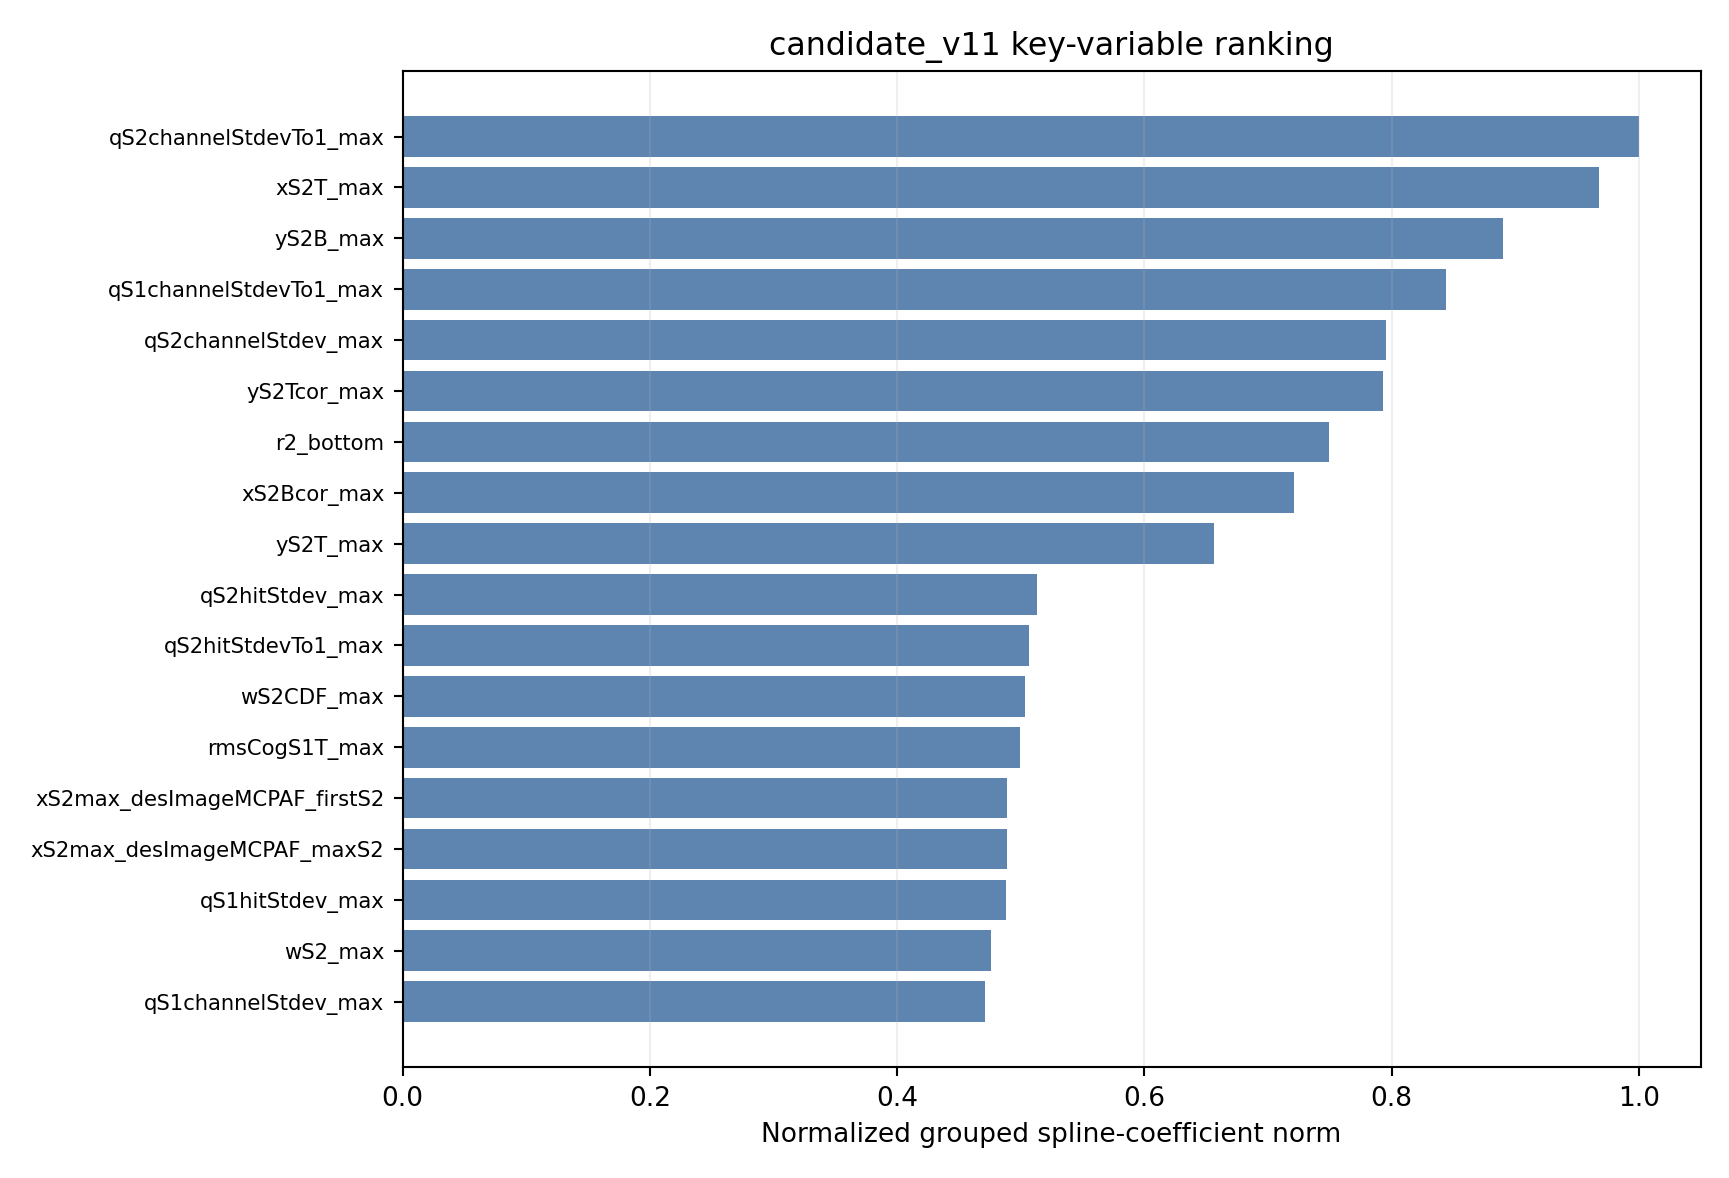
\includegraphics[width=0.91\textwidth]{v11_feature_importance.png}
\caption{candidate\_v11 的置换重要性。横轴越大，打乱该参量后性能损失越明显。}
\end{figure}

\begin{table}[H]
\centering
\caption{重要性最高的五个参量}
\begin{tabularx}{0.9\textwidth}{cYc}
\toprule
排名 & 参量 & 相对重要性\\
\midrule
1 & \var{qS2channelStdevTo1_max} & 1.000\\
2 & \var{xS2T_max} & 0.968\\
3 & \var{yS2B_max} & 0.890\\
4 & \var{qS1channelStdevTo1_max} & 0.844\\
5 & \var{qS2channelStdev_max} & 0.796\\
\bottomrule
\end{tabularx}
\end{table}

\begin{keybox}
\textbf{解释：}关键参量主要来自 S2/S1 通道图样与横向位置，说明峰宽中有相当部分
来自光收集空间不均匀和通道分布差异。重要性反映预测贡献，不等于因果关系。
\end{keybox}

\clearpage
\section{模型改进幅度}

\begin{figure}[H]
\centering
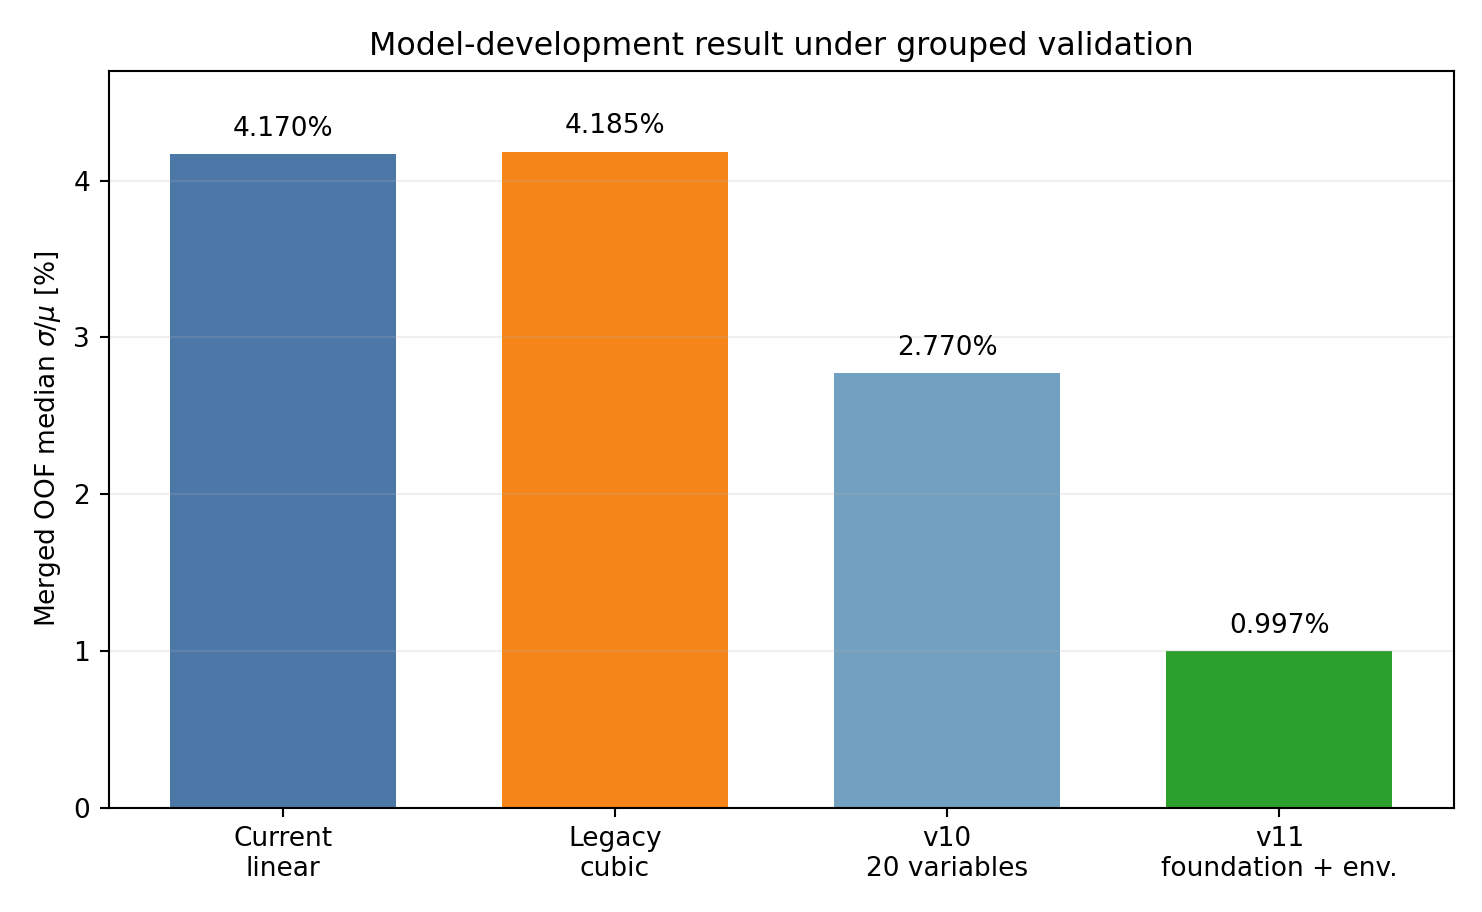
\includegraphics[width=0.91\textwidth]{v11_model_progress.png}
\caption{不同重建方案在同一数据上的分辨率比较，数值越低越好。}
\end{figure}

\begin{table}[H]
\centering
\caption{核心方案对比}
\begin{tabular}{l c}
\toprule
方案 & 合并 OOF \(\sigma/\mu\)\\
\midrule
当前线性公式 & \(4.1696\%\)\\
已有三次多项式修正 & \(4.1847\%\)\\
训练侧选择的 foundation & \(3.8552\%\)\\
candidate\_v10 & \(2.7698\%\)\\
\rowcolor{SoftTeal}\textbf{candidate\_v11} & \(\mathbf{0.9973\%}\)\\
\bottomrule
\end{tabular}
\end{table}

\begin{resultbox}
v11 的主要提升来自两点：一是先在训练侧选择更合适的 S1/S2 基础信号；
二是加入能够描述通道图样、位置和事件环境的参量，并通过样条 Ridge 做受控的非线性修正。
\end{resultbox}

\clearpage
\section{一维能谱结果}

\begin{figure}[H]
\centering
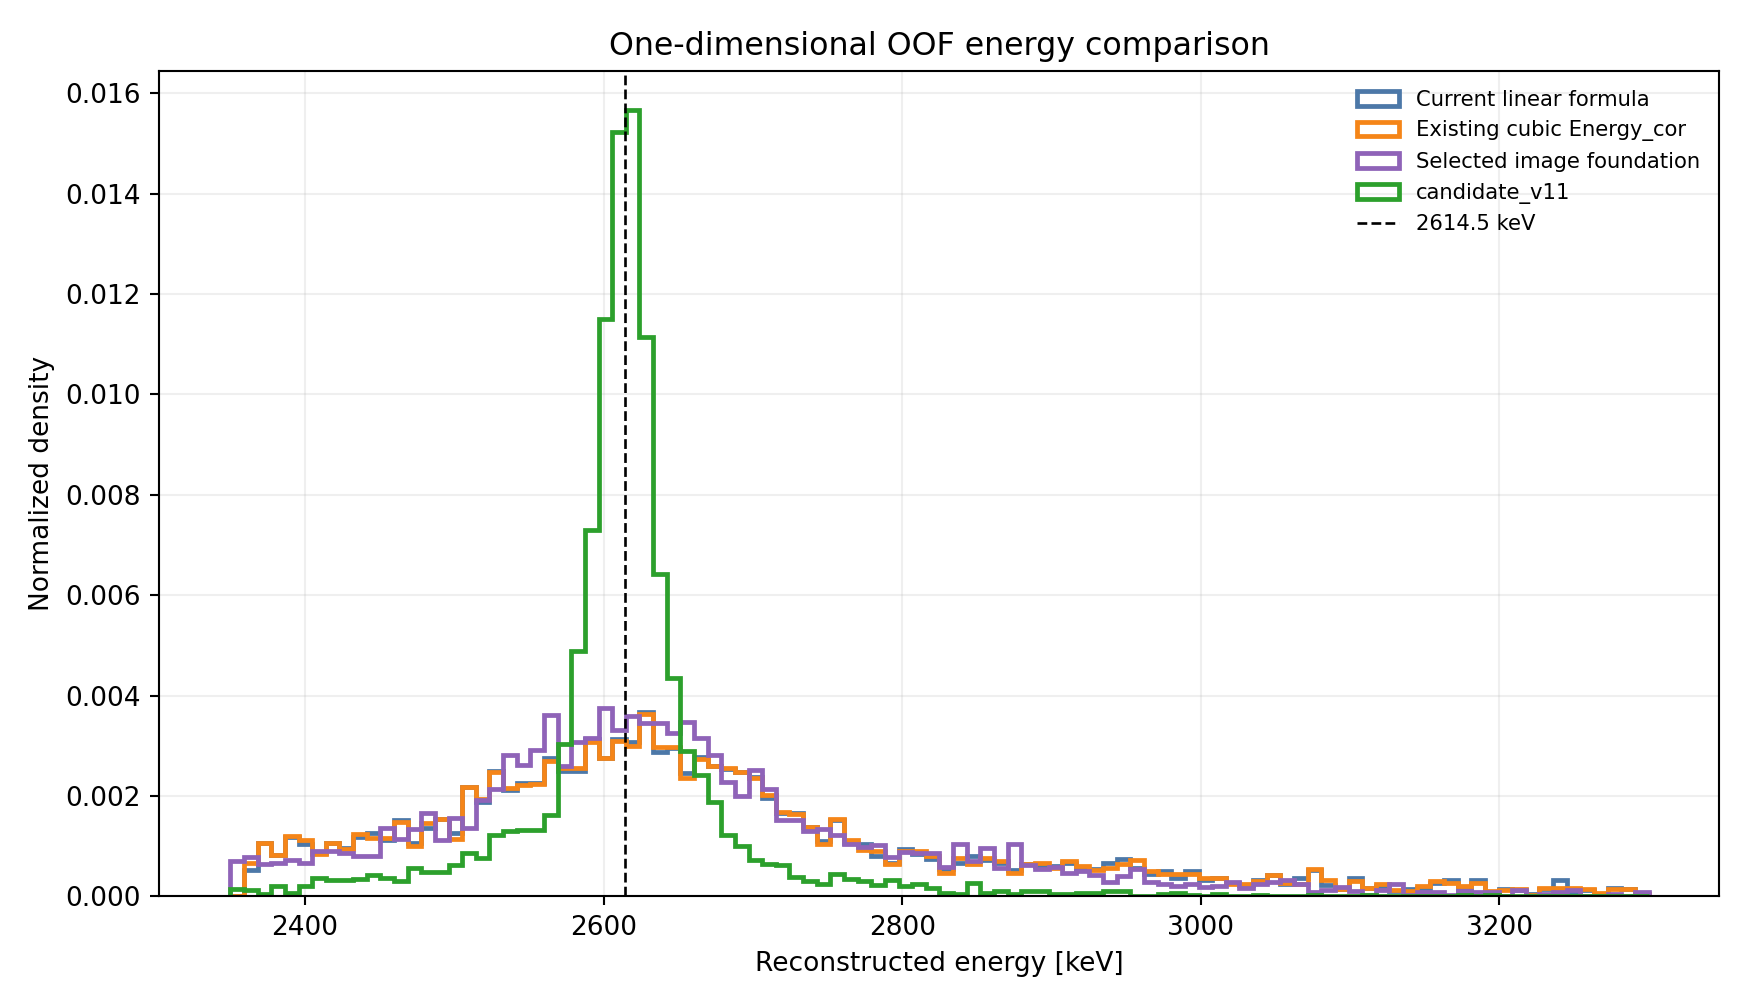
\includegraphics[width=0.93\textwidth]{v11_energy_1d.png}
\caption{不同方案的一维能量分布。v11 的峰核心明显更集中。}
\end{figure}

\begin{table}[H]
\centering
\caption{candidate\_v11 的主要宽度指标}
\begin{tabular}{l c}
\toprule
指标 & 结果\\
\midrule
高斯核心宽度 \(\sigma/\mu\) & \(0.9973\%\)\\
最差外层块 \(\sigma/\mu\) & \(1.0427\%\)\\
中心 68\% 半宽 \(R_{68}\) & \(1.3674\%\)\\
中心 90\% 半宽 \(R_{90}\) & \(4.2483\%\)\\
峰中心最大相对偏差 & \(0.0168\%\)\\
\bottomrule
\end{tabular}
\end{table}

\begin{warnbox}
\textbf{不能只看 \(\sigma/\mu\)：}当前高斯拟合的 \(p\) 值中位数接近 0，
说明峰形并非理想高斯。因此同时报告 \(R_{68}\)、\(R_{90}\) 与分块稳定性，
避免把“核心变窄”误当成“所有尾部都消失”。
\end{warnbox}

\clearpage
\section{分块稳定性}

\begin{figure}[H]
\centering
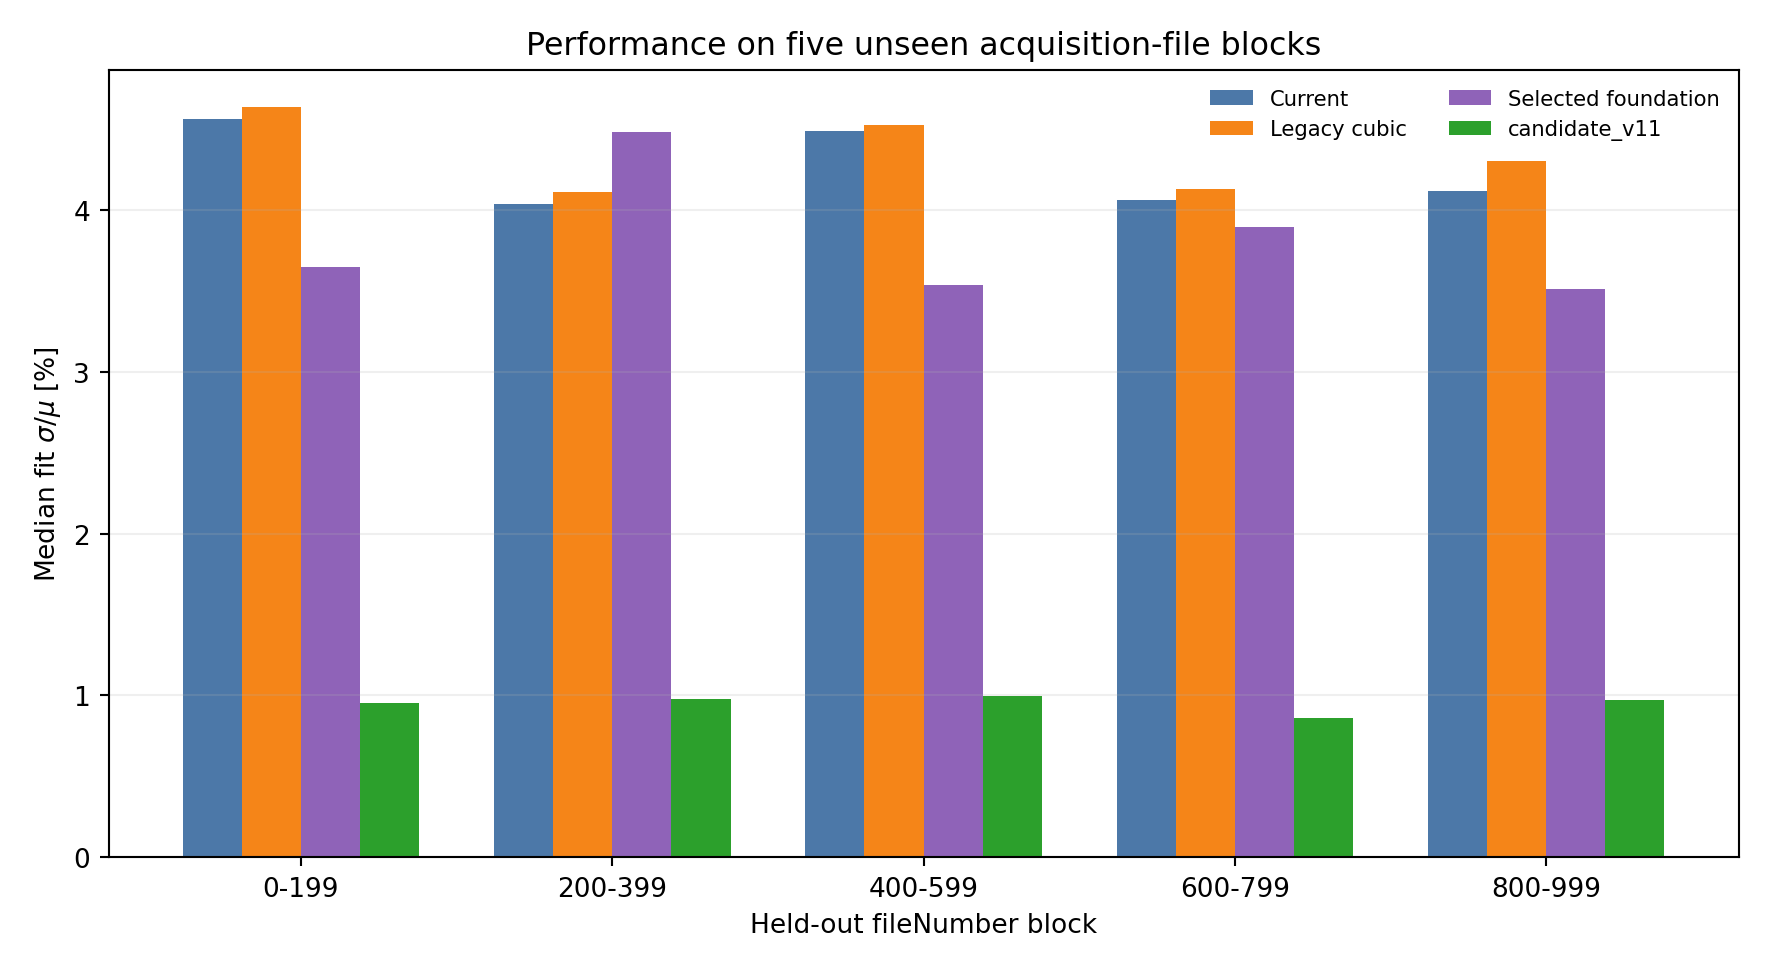
\includegraphics[width=0.92\textwidth]{v11_outer_blocks.png}
\caption{五个未见文件块上的 \(\sigma/\mu\)。每一块都没有参与该轮模型训练。}
\end{figure}

\begin{table}[H]
\centering
\caption{五个完整文件块的结果}
\begin{tabular}{c c c}
\toprule
外层块 & \var{fileNumber} 范围 & \(\sigma/\mu\)\\
\midrule
1 & 0--199 & \(0.9523\%\)\\
2 & 200--399 & \(0.9774\%\)\\
3 & 400--599 & \(0.9990\%\)\\
4 & 600--799 & \(0.8595\%\)\\
5 & 800--999 & \(0.9701\%\)\\
\bottomrule
\end{tabular}
\end{table}

\begin{resultbox}
五块结果均低于 \(1.00\%\)，最差块为 \(1.0427\%\) 的更保守统计口径；
这说明改善不是由某一个局部文件段单独贡献。不过它们仍属于同一个 Run 10972，
不能替代独立新 run 的盲测。
\end{resultbox}

\clearpage
\begin{landscape}
\section{二维位置残差}
\begin{figure}[H]
\centering
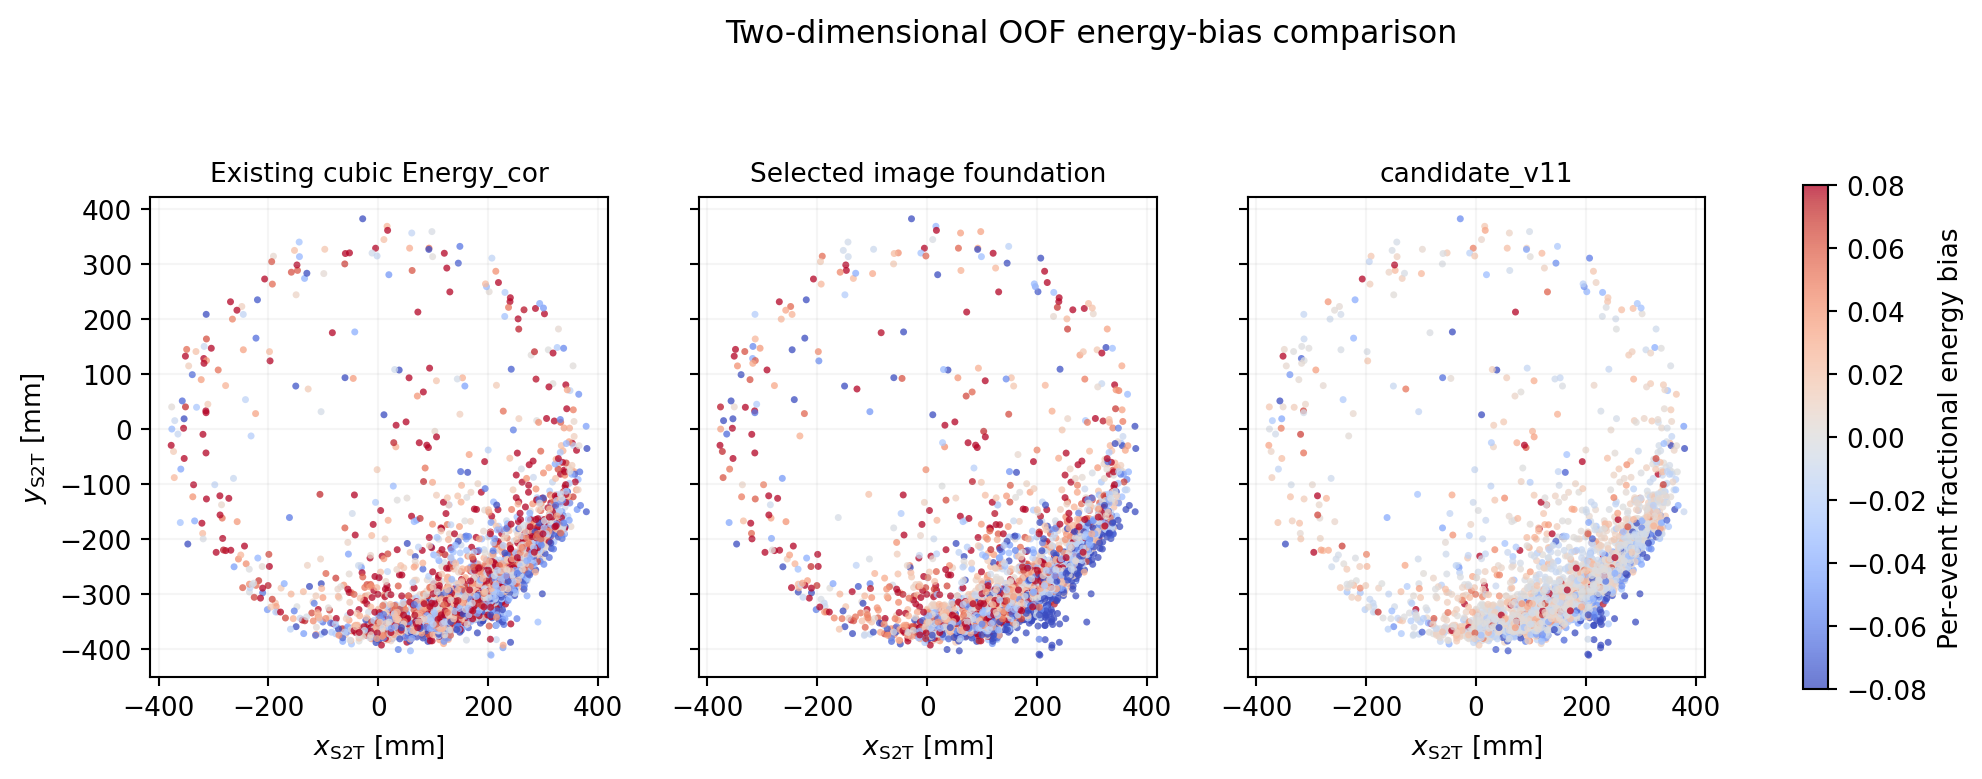
\includegraphics[width=0.88\linewidth]{v11_xy_bias.png}
\caption{修正后能量在 \(x\)--\(y\) 平面上的相对偏差。颜色表示局部峰中心相对整体中心的偏移。}
\end{figure}
\begin{keybox}
这张图检查模型是否只在总体上变窄、却在某些位置留下系统偏差。
当前峰中心最大相对偏差约为 \(0.0168\%\)，未观察到明显的大尺度位置结构；
低统计区域仍应在新数据上重点检查。
\end{keybox}
\end{landscape}

\clearpage
\section{修正强度与最终结论}

\begin{figure}[H]
\centering
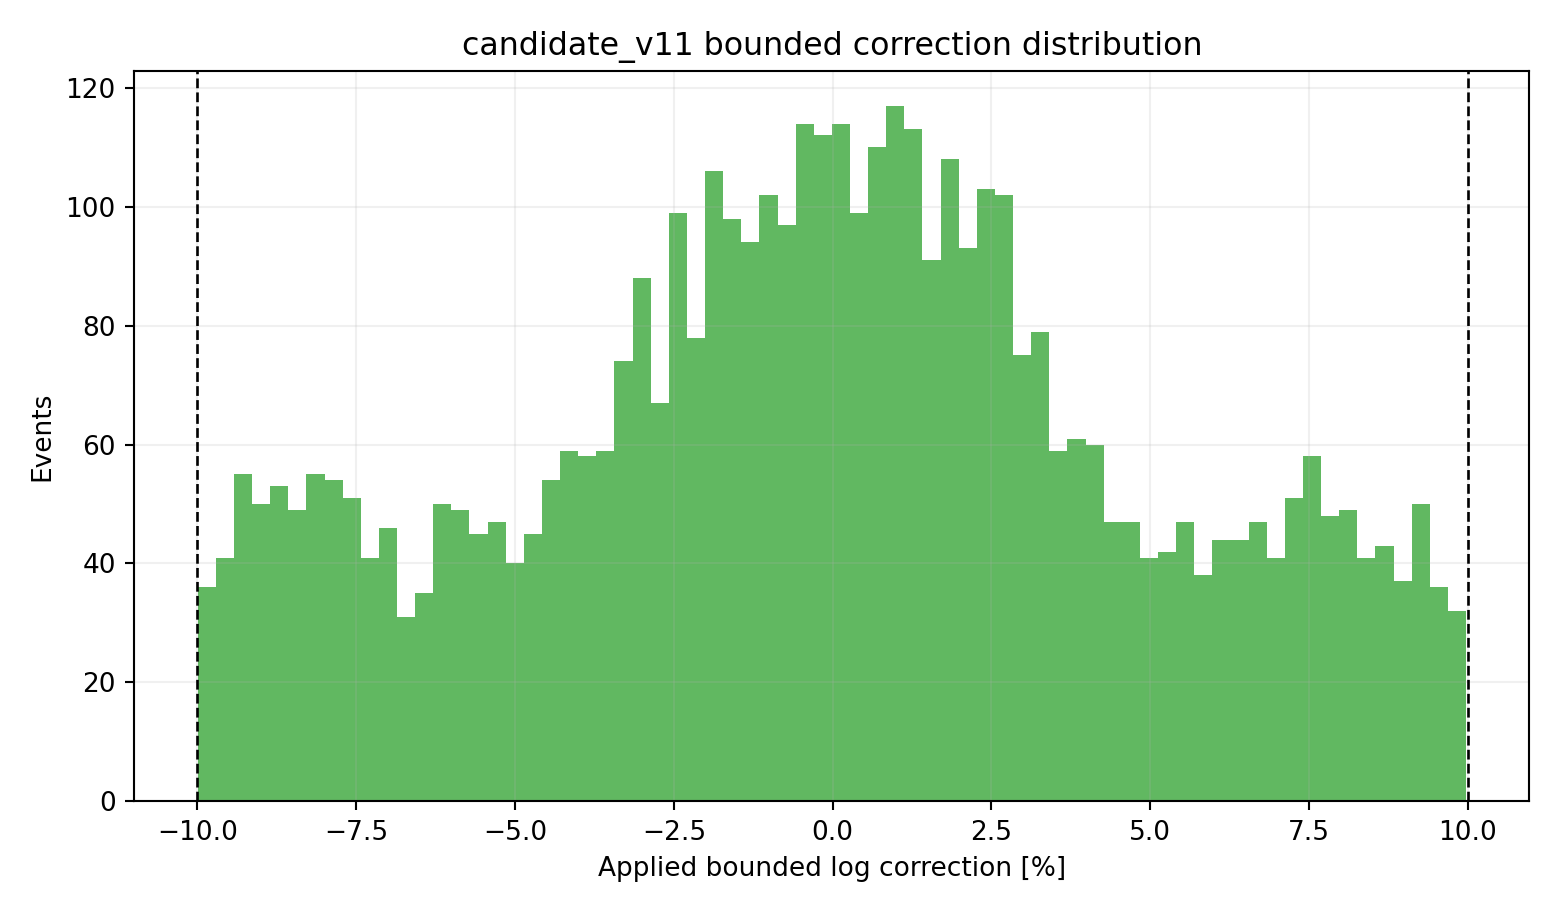
\includegraphics[width=0.9\textwidth]{v11_correction.png}
\caption{逐事件对数修正 \(\delta\) 的分布及截断情况。}
\end{figure}

\begin{itemize}
  \item 修正采用 \(0.10\tanh(\cdot/0.10)\) 软限制，避免极端外推。
  \item 约 \(2.60\%\) 的事件接近修正上限，说明仍有少量难以描述的尾部事件。
  \item 模型、训练中位数、特征顺序和参数已封装，可直接用于老师的新数据盲测。
\end{itemize}

\begin{resultbox}
\textbf{最终做到的事情：}
我们从 S1/S2 基础能量出发，建立了一个使用 64 个受控参量的样条 Ridge 修正模型；
在 Run 10972 的文件分组 OOF 验证中得到 \(0.9973\%\) 的核心分辨率，
且五个外层块保持稳定。下一步唯一关键任务，是在完全独立的新 run 上冻结模型盲测：
若峰中心、\(R_{68}\)、\(R_{90}\) 和分块稳定性仍同时改善，才能确认模型具有可迁移性。
\end{resultbox}

\begin{warnbox}
\textbf{结论边界：}candidate\_v11 是目前内部验证最好的候选模型，
不是已经证明的全局最优模型，也不应把 \(0.9973\%\) 直接表述为最终物理结果。
\end{warnbox}

\end{document}
